Start de LibreOffice Writer applicatie op.

Neem de tekst over uit de plaat in figuur \ref{fig:LOWriter_tekst} en zorg dat deze tekst een hoofdstuk titel wordt door de stijl te
veranderen. We gaan het document later vullen. Selecteer File en Save as{\dots} om het bestand op te slaan met als naam:
Document1. Sluit daarna LibreOffice Writer weer af.

\begin{figure}[H]
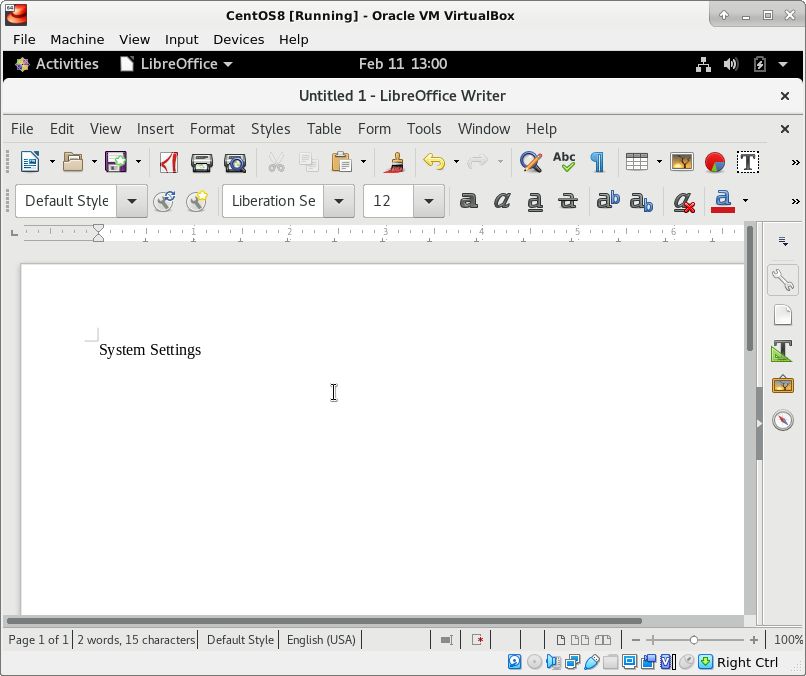
\includegraphics[width=0.9\textwidth]{linuxreader-img015.png}
	\caption{LibreOffice Writer met een eerste tekts}
	\label{fig:LOWriter_tekst}
\end{figure}
